% Unofficial SDU AI Poster Template
% v1.0.0 released Octobor 17, 2023
% https://github.com/k4rtik/uchicago-poster
% a fork of https://github.com/anishathalye/gemini

\documentclass[final]{beamer}

% ====================
% Packages
% ====================

\usepackage[T1]{fontenc}
\usepackage{lmodern}
%\usepackage[size=custom,width=120,height=72,scale=1.0]{beamerposter}
\usepackage[orientation=portrait, size=a0, scale=1, debug]{beamerposter}
\usetheme{gemini}
\usecolortheme{technion}

\usepackage[caption=false,font=normalsize,labelfont=sf,textfont=sf]{subfig}
\usepackage{graphicx}
\usepackage{booktabs}
\usepackage{doi}
\usepackage[numbers]{natbib}
\usepackage[patch=none]{microtype}
\usepackage{tikz}
\usepackage{pgfplots}
\pgfplotsset{compat=1.18}
\usepackage{anyfontsize}
\usepackage{multirow}

\pdfstringdefDisableCommands{%
	\def\translate#1{#1}%
}

% ====================
% Lengths
% ====================

% If you have N columns, choose \sepwidth and \colwidth such that
% (N+1)*\sepwidth + N*\colwidth = \paperwidth
\newlength{\sepwidth}
\newlength{\colwidth}
\setlength{\sepwidth}{0.025\paperwidth}
\setlength{\colwidth}{0.3\paperwidth}

\newcommand{\separatorcolumn}{\begin{column}{\sepwidth}\end{column}}
\newcommand{\mymethodname}{SDOH-HC}


% ====================
% Title
% ====================

\title{Self-Distillation Dual-Memory Online Hashing with \\ Hash Centers for Streaming Data Retrieval}

\author{Chong-Yu Zhang \inst{1}, Xin Luo \inst{1*}, Yu-Wei Zhan \inst{1}, Peng-Fei Zhang \inst{2}, Zhen-Duo Chen \inst{1}, Yongxin Wang \inst{3}, Xun Yang \inst{4}, Xin-Shun Xu \inst{1}}

\institute[shortinst]{\inst{1} Shandong University \samelineand \inst{2} University of Queensland \samelineand \inst{3} Shandong Jianzhu University    \samelineand \inst{4} University of Science and Technology}

% ====================
% Footer (optional)
% ====================

\footercontent{
	* Corresponding author, luoxin.lxin@gmail.com. \hfill
	$31^{th}$ ACM Multimedia, October 29-November 3, 2023, Ottawa, ON, Canada \hfill
	\href{mailto:zhangchongyu22@gmail.com}{zhangchongyu22@gmail.com}}


% ====================
% Logo (optional)
% ====================

% use this to include logos on the left and/or right side of the header:
% \logoright{\includegraphics[height=7cm]{logo1.pdf}}
% \logoleft{\includegraphics[height=7cm]{logo2.pdf}}

% ====================
% Body
% ====================

\begin{document}
	\addtobeamertemplate{headline}{}
	{
		\begin{tikzpicture}[remember picture,overlay]
			\node [anchor=north west, inner sep=1cm] at ([xshift=1.0cm, yshift=-0.5cm]current page.north west)
			{\includegraphics[height=5.0cm]{logos/mm2023_unofficial.png}}; % also try shield-white.eps
			
			\node [anchor=north east, inner sep=0cm] at ([xshift=-10.3cm,yshift=-1cm]current page.north east)
			{\includegraphics[height=6cm]{logos/c2.png}};
			
			\node [anchor=north east, inner sep=0cm] at ([xshift=-7.8cm,yshift=-2cm]current page.north east)
			{\includegraphics[height=4cm]{logos/uq.png}};
			
			\node [anchor=north east, inner sep=0cm] at ([xshift=-3.5cm,yshift=-2cm]current page.north east)
			{\includegraphics[height=4cm]{logos/sdjzu.png}};
			
			\node [anchor=north east, inner sep=0cm] at ([xshift=0.0cm,yshift=-2.0cm]current page.north east)
			{\includegraphics[height=4.0cm]{logos/ustc.png}};
			
			\node [anchor=north east, inner sep=1cm] at ([xshift=0.0cm,yshift=-6cm]current page.north east)
			{\includegraphics[height=4.0cm]{logos/code.png}};
		\end{tikzpicture}
	}
	
	\begin{frame}[t]
		\begin{columns}[t]
			\separatorcolumn
			
			\begin{column}{\colwidth}
				
				\begin{block}{Introduction}
					
					With the continuous generation of massive amounts of multimedia data nowadays, hashing has demonstrated significant potentials for large-scale search. To handle the emerging needs for streaming data retrieval, online hashing is drawing more and more attention. For online scenario, data distribution may change and concept drifts may occur as new data is continuously added to the database. Inevitably, hashing models may lose or disrupt the previously obtained knowledge when learning from new information, which is called the problem of \textbf{catastrophic forgetting}. In this paper, we propose a new online hashing method called Self-distillation Dual-memory Online Hashing with Hash Centers, which is abbreviated to \mymethodname, to overcome this challenge. Specifically, \mymethodname~ contains replay and distillation modules. For replay, a dual-memory mechanism is proposed which involves hash centers and exemplars. For knowledge distillation, we let hash centers distill information from themselves, i.e., the version of last round. Additionally, a new objective function is further built on above modules and is solved discretely to learn hash codes. Extensive experiments on three benchmark datasets demonstrate the effectiveness of our method.
					
				\end{block}
				
				\begin{block}{The Proposed Method}
					\textbf{Notations and Problem Definition}
					
					In this paper, we assume that the image data comes at a streaming manner. At the $t$-th round. A new chunk of image data $ \vec{\mathbf{X}}^{(t)} \in \mathbb{R}^{n_t \times d}$ is added to the database, where $n_t$ is the chunk size and $d$ is the feature dimensionality. $ \vec{\mathbf{L}}^{(t)} \in \mathbb{R}^{n_t \times c}$ is the corresponding label matrix of new chunk, where $c$ is the number of categories. Before this chunk, existing old data at previous rounds $\tilde{\mathbf{X}}^{(t)} \in \mathbb{R}^{N_{t-1} \times d}$ (with labels $\tilde{\mathbf{L}}^{(t)} \in \mathbb{R}^{N_{t-1} \times c}$) have been used for training and accumulated in the database, and the corresponding hash codes $\tilde{\mathbf{B}}^{(t)} \in \{-1, 1\}^{N_{t-1} \times r} $ have also been generated and stored, where $N_{t-1} = n_1+,...,+n_{t-1}$ is the size of existing data and $r$ is the length of hash codes.
					
					For online hashing, the goals are: 1) generating hash codes  $\vec{\mathbf{B}}^{(t)}  $ for newly coming data; 2) learning the hash function matrix $\mathbf{P}^{(t)}$ which could transform query data $\mathbf{q}$ into hash codes by $ sgn(\mathbf{q}\mathbf{P}^{(t)})$. 
					
					
					\textbf{Hash Centers Calculation}
					
					The concept of \textbf{hash center} is recently proposed in \cite{yuan2020central} for the first time, which refers to a set of data points scattered in the Hamming space with a sufficient mutual distance between each other. However, fixed hash centers extracted via predetermined Hadamard matrix \cite{lin2020hadamard} may be suboptimal  because they contain no semantic information and could not properly adapt to the data distribution. In online hashing, how to learn non-fixed hash centers is still an open problem. Besides, the stability-plasticity dilemma \cite{robins1995catastrophic} should be well taken into consideration. If we use fixed hash centers, models may fail to be plastic enough to adapt to changing environments and learn new knowledge from streaming data. How to let hash centers achieve an appropriate balance between stability and plasticity has not been investigated.
					
					To overcome above limitations, we propose a novel and new hash centers calculation strategy, which can be written as follows,
					
					\begin{equation}
						\begin{aligned}
							& \min_{\vec{\mathbf{B}}^{(t)},\vec{\mathbf{Y}}^{(t)}}
							\theta \|\mathbf{C}- \vec{\mathbf{Y}}^{(t)T}\|_{F}^{2} + \eta \| r \vec{\mathbf{L}}^{(t)} - \vec{\mathbf{B}}^{(t)} \vec{\mathbf{Y}}^{(t)T} \|_F^2, \\
							&s.t. \ \ \vec{\mathbf{B}}^{(t)} \in \{-1,1\}^{n_{t} \times r}, \vec{\mathbf{Y}}^{(t)} \in   \{-1, 1\}^{c \times r},
						\end{aligned}
						\label{pro_smi_embedding}
					\end{equation}
					where $\mathbf{C} \in \{-1,1\}^{r \times c}$ is the predetermined hash centers based on Hadamard matrix, $\vec{\mathbf{Y}}^{(t)} \in \{-1,1\}^{c \times r}$ is the learnable hash centers at $t$-th round, which is not fixed and could adapt to newly arriving data, $\theta$ and $\eta$ are trade-off parameters. For the first term, we let $\vec{\mathbf{Y}}^{(t)}$ be similar with the fixed hash centers $\mathbf{C}$. There are several advantages: 1) Hadamard matrix based hash centers could act as good initialization of $\vec{\mathbf{Y}}^{(t)}$; 2) $\vec{\mathbf{Y}}^{(t)}$ is possible to inherit the good property from $\mathbf{C}$ that hash centers in $\mathbf{C}$ are mutually orthogonal; 3) as $\mathbf{C}$ is fixed while $\vec{\mathbf{Y}}^{(t)}$ is learnable, we expect $\vec{\mathbf{Y}}^{(t)}$ to be stable and plastic enough by making them similar. For the second term, the connection between hash centers and hash codes of data is built. If two samples share the same labels, they will have the same hash codes which meets the core of hash learning that semantically similar samples should be close in Hamming space.
					
					
					\textbf{Self-Distillation Loss}
					
					Following the teacher-student distillation paradigm, we take a different approach that we denote the hash centers of last round as  $\tilde{\mathbf{Y}}^{(t)}$ ($\tilde{\mathbf{Y}}^{(t)}$ can also be represented as $\vec{\mathbf{Y}}^{(t-1)}$) and enable it to act as the teacher to guide the learning of $\vec{\mathbf{Y}}^{(t)}$. The formulation can be represented as follows, 
					
					\vspace{-2mm}

					\begin{equation}
						\begin{aligned}
							& \min_{\vec{\mathbf{Y}}^{(t)}}
							\  \| r\mathbf{K}-\tilde{\mathbf{Y}}^{(t)}  \vec{\mathbf{Y}}^{(t)T} \|_{F}^{2}\ \  s.t. \  \vec{\mathbf{Y}}^{(t)} \in   \{-1, 1\}^{c \times r},
						\end{aligned}
						\label{Self-Distillation Loss}
						\vspace{-1mm}
					\end{equation}
					where $\mathbf{K}$ is the constructed pairwise similarity matrix among hash centers. In matrix $\mathbf{K}$ whose size is c$\times$c, the diagonal elements are all 1 while the remaining elements are -1 since every class is not similar with others but itself.
					
					From  Eq. (\ref{Self-Distillation Loss}), only former and current hash centers are involved. This loss can be viewed as that we use former hash centers as teacher to guide the learning of student.  Thus, we call this different knowledge distillation term as \textbf{self-distillation}.

					
				\end{block}
				
			\end{column}
			
			\separatorcolumn
			
			\begin{column}{\colwidth}
				
					\textbf{Hash Center and Exemplar Memories}
					
					To support self-distillation in Eq. (\ref{Self-Distillation Loss}), a \textbf{hash center memory} is used to dynamically store the hash centers at each data round. Besides, a subset of representative data points are stored in \textbf{exemplar memory} to further alleviate catastrophic forgetting. We retain the similarity between exemplars and new data samples, and try to embed the knowledge behind exemplars into the hash codes learning procedure of new data,
					
					\vspace{-3mm}
					\begin{equation}
						\begin{aligned}
							\min_{\vec{\mathbf{B}}^{(t)}} \| r\mathbf{S}_{qn}^{(t)} - \tilde{\mathbf{B}}^{(t)}_{q}\vec{\mathbf{B}}^{(t)} \|_{F}^{2}  \ \ 
							s.t. \ \vec{\mathbf{B}}^{(t)} \in \{-1,1\}^{n_{t} \times r},
						\end{aligned}
						\label{memory-newdata}
						\vspace{-1mm}
					\end{equation}
					where $\mathbf{S}_{qn}^{(t)}$ is the constructed similarity and $\tilde{\mathbf{B}}^{(t)}_{q}$ is the hash codes of exemplars which is stored in memory. Besides, we design a novel calculation of $\mathbf{S}_{qn}^{(t)}$. If one exemplar and one new data point is semantically dissimilar, we directly assign the value -1 to measure their similarity. Otherwise, if they are semantically similar, the similarity is defined as the inner product of their features.
					
					In the exemplar memory, information of $n_{q}$ points are saved. The exemplar memory is dynamically updated. At each round, $n_{2}$ points are selected from new data chunk to replenish the exemplar memory and we randomly retain $n_{1}$ points from $n_{q}$ points, where $n_{q}= n_{1}+ n_{2}$. For point selection strategy, please refer to the paper.
%					we turn to the second term in Eq. \eqref{pro_smi_embedding} for help. This term forces semantically similar sample to have similar hash codes and serves the goal of similarity-preserving. Thus, we choose to pick up points, which have smaller values of this term.


					\begin{block}{Overall Architecture}
						\begin{figure}
							\centering
							\includegraphics[width=1\colwidth]{figures/MM_SDOH-HC-framework}
							\vspace{-2cm}
							\caption{The overall framework of \mymethodname. The pink region illustrates hash codes learning step while the beige region represents hash function learning step. Within hash codes learning, mistyrose and lightcyan areas are hash centers self-distillation and exemplar memory, respectively.} 
							\label{framework}
							\vspace{-1.2cm}
						\end{figure}
					\end{block}




					\textbf{Hashing Formulation}
					
					
					Within the supervised hashing literature, the $\|r\mathbf{S}-\mathbf{B}\mathbf{B}\|_{F}^{2}$ term is widely employed to preserve semantic similarity, where $\mathbf{S}$ denotes the instance-instance pairwise similarity matrix of the data. We employ a subtle method to construct $\mathbf{S}$ to avoid square time complexity, i.e., $\mathbf{S} = {\mathbf{L}} {\mathbf{L}}^{T}$, where ${\mathbf{L}}$ represents the $\ell_{2}$-norm of the normalized label matrix, with the $j$-th row defined as $\mathbf{L}_{j} = \mathbf{L}_{j}/\|\mathbf{L}_{j}\|$. To accommodate the online scenario, at the $t$-th round, $\mathbf{S}^{(t)}$ can be reformulated as follows,
					
					\vspace{-3mm}
					
					\begin{equation}
						\begin{aligned}
							\mathbf{S^{(t)}} = \begin{bmatrix}  \mathbf{S}_{oo}^{(t)}& \mathbf{S}_{on}^{(t)}\\  \mathbf{S}_{no}^{(t)}& \mathbf{S}_{nn}^{(t)}\end{bmatrix},
						\end{aligned}
						\label{S_online_scenario}
					\end{equation}
					where letter `o' in subscript represents old data and `n' denotes new data. For example, $\mathbf{S}_{no}^{(t)}$ means the similarity between new data and old data at current round.
					
					
					For the sake of simplicity, we solely utilize $\mathbf{S}_{no}^{(t)}$. Therefore, the hashing formulation can be reformulated as follows,
					\begin{equation}
						\begin{aligned}
							& \min_{\vec{\mathbf{B}}^{(t)}}	\| r\mathbf{S}_{no}^{(t)} - \vec{\mathbf{B}}^{(t)} \tilde{\mathbf{B}}^{(t)T} \|_{F}^{2}, \ \
							s.t. \vec{\mathbf{B}}^{(t)} \in \{-1,1\}^{n_{t} \times r}.
						\end{aligned}
						\label{Sno_SBB}
					\end{equation}
					In this equation, by minimizing the squared loss between the similarity matrix of old and new data and the inner product of the hash codes, knowledge acquired in the past is embedded into the hash codes of new data.
					
					Considering the NP-hard optimization problem, we employ a real-valued auxiliary variable $\mathbf{V}$ as a substitute for hash codes. Meanwhile, the constraint of $\mathbf{V} \mathbf{V} = n \mathbf{I}_{r}$ is added to ensure that each bit represents as much information as possible, while the $\mathbf{V}\mathbf{1} = \mathbf{0}_{r}$ constraint is given to enhance the discriminative power of the hash codes. We simultaneously rewrite Eq. \eqref{memory-newdata} and Eq. \eqref{Sno_SBB} can be rewritten as follows,
					%\vspace{-1mm}
					\begin{equation}
						\begin{aligned}
							&\min_{\vec{\mathbf{B}}^{(t)},\vec{\mathbf{V}}^{(t)}} \| r\mathbf{S}_{no}^{(t)} - \vec{\mathbf{B}}^{(t)} \tilde{\mathbf{V}}^{(t)T} \|_{F}^{2} + \| r\mathbf{S}_{qn}^{(t)} - \tilde{\mathbf{B}}^{(t)}_{q} \vec{\mathbf{V}}^{(t)T} \|_{F}^{2} \\
							&+ \beta \| \vec{\mathbf{B}}^{(t)} -\vec{\mathbf{V}}^{(t)} \|_{F}^{2} \ \  s.t. \  \vec{\mathbf{B}}^{(t)} \in \{-1,1\}^{n_{t} \times r},\vec{\mathbf{Y}}^{(t)} \in  \\
							&  \{-1, 1\}^{c \times r},  \vec{\mathbf{V}}^{(t)}\vec{\mathbf{V}}^{(t)T} = n_{t} \mathbf{I}_{r}, \vec{\mathbf{V}}^{(t)}\mathbf{1} = \mathbf{0}_{r},
						\end{aligned}
						\label{hashformulation}
					\end{equation}
					where $\beta$ is a trade-off parameter.
					
				
				
				
				

				\begin{block}{Overall Objective Function}
					
					In summary, our \mymethodname~is built based on hash centers and two memories with distillation and replay. By combining Eq. \eqref{pro_smi_embedding}, Eq. \eqref{Self-Distillation Loss}, and Eq. \eqref{hashformulation}, we could obtain its overall loss function,
					\begin{equation}
						\begin{aligned}
							&\min_{\vec{\mathbf{B}}^{(t)},\vec{\mathbf{V}}^{(t)},\vec{\mathbf{Y}}^{(t)}} \| r\mathbf{S}_{no}^{(t)} - \vec{\mathbf{B}}^{(t)} \tilde{\mathbf{V}}^{(t)T} \|_{F}^{2} + \| r\mathbf{S}_{qn}^{(t)} - \tilde{\mathbf{B}}^{(t)}_{q} \vec{\mathbf{V}}^{(t)T} \|_{F}^{2} \\
							&+ \beta \| \vec{\mathbf{B}}^{(t)}-\vec{\mathbf{V}}^{(t)} \|_{F}^{2} + \theta (\| r\mathbf{K}-\tilde{\mathbf{Y}}^{(t)}  \vec{\mathbf{Y}}^{(t)T} \|_{F}^{2} +\|\mathbf{C}- \vec{\mathbf{Y}}^{(t)T}\|_{F}^{2} ) \\
							&+ \eta \| r \vec{\mathbf{L}}^{(t)} - \vec{\mathbf{B}}^{(t)} \vec{\mathbf{Y}}^{(t)T}  \|_F^2, \ \ \  s.t. \  \vec{\mathbf{B}}^{(t)} \in \{-1,1\}^{n_{t} \times r},\vec{\mathbf{Y}}^{(t)} \in  \\
							&  \{-1, 1\}^{c \times r},  \vec{\mathbf{V}}^{(t)}\vec{\mathbf{V}}^{(t)T} = n_{t} \mathbf{I}_{r}, \vec{\mathbf{V}}^{(t)}\mathbf{1} = \mathbf{0}_{r}.
						\end{aligned}
						\label{overallobjectivefunction}
					\end{equation}
					
					
					
					
				\end{block}
				
				
				
			\end{column}
			
			\separatorcolumn
			
			\begin{column}{\colwidth}
				
				\begin{block}{Experiment}
					\textbf{Datasets}
					
					Three benchmark datasets are chosen for evaluation, i.e., CIFAR-10, MIRFlickr, and NUS-WIDE, the last two of which are multi-label datasets. When evaluating, two samples are viewed as similar if they correspond to the same label on CIFAR-10. For multi-label datasets MIRFlickr and NUS-WIDE, two samples are considered similar if they share at least one common label.
					
					\textbf{Evaluation Metrics}
					
					Following existing online hashing literature, we employed two widely-used metrics, namely mean average precision (MAP) and precision-recall (P-R) curves, to evaluate the efficacy. Higher MAP scores indicate superior performance and larger areas under the P-R curves signify more favorable outcomes.
					
					\textbf{Comparison with Baselines}
					
					\begin{figure}
						\centering
						\captionsetup[subfloat]{labelformat=empty}
						\subfloat[]{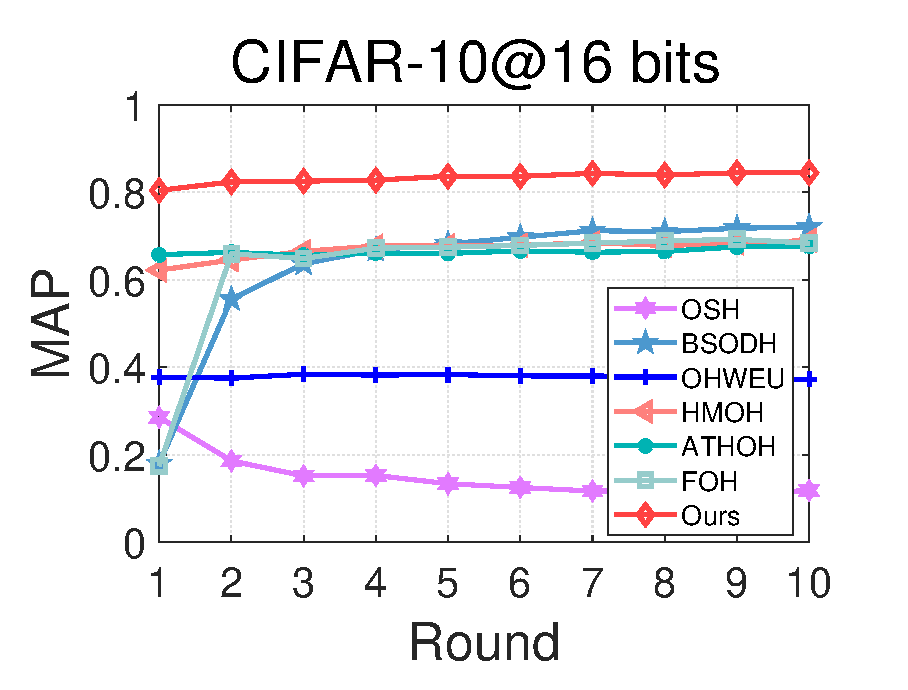
\includegraphics[width=0.3\columnwidth]{figures/map_round/CIFAR-10@16bits}
							\label{fig:CIFAR-10@16bits}}
						\subfloat[]{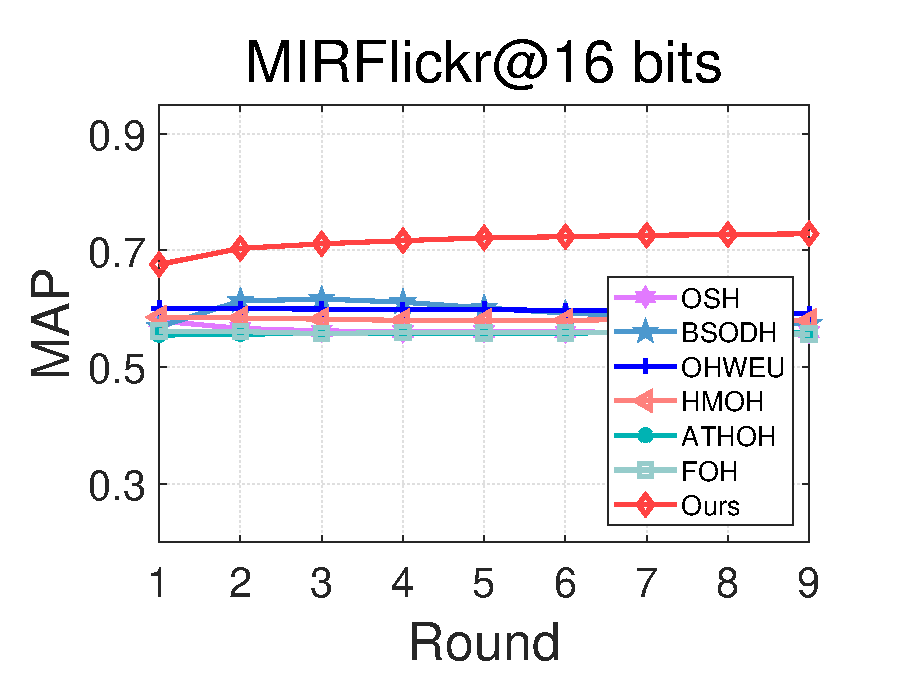
\includegraphics[width=0.3\columnwidth]{figures/map_round/MIRFlickr@16bits}
							\label{fig:MIRFlickr@16bits}}
						\subfloat[]{\includegraphics[width=0.3\columnwidth]{figures/map_round/NUS-WIDE@16bits}
							\label{fig:NUS-WIDE@16bits}}
						\vspace{-5mm}
						\quad
						\vspace{-5mm}
						\subfloat[]{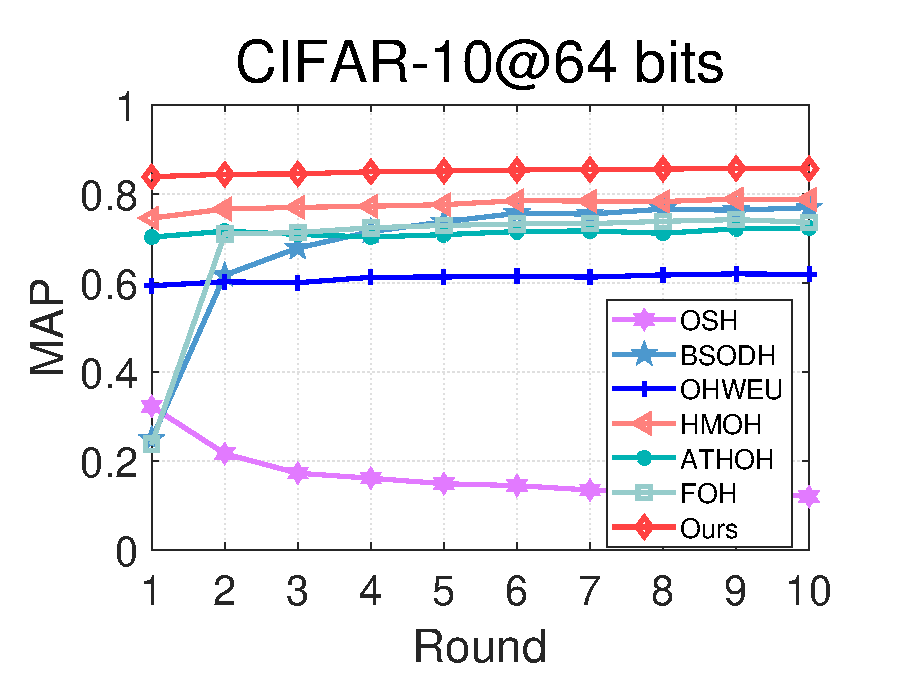
\includegraphics[width=0.3\columnwidth]{figures/map_round/CIFAR-10@64bits}
							\label{fig:CIFAR-10@64bits}} 
						%	\vspace{-2mm}
						\subfloat[]{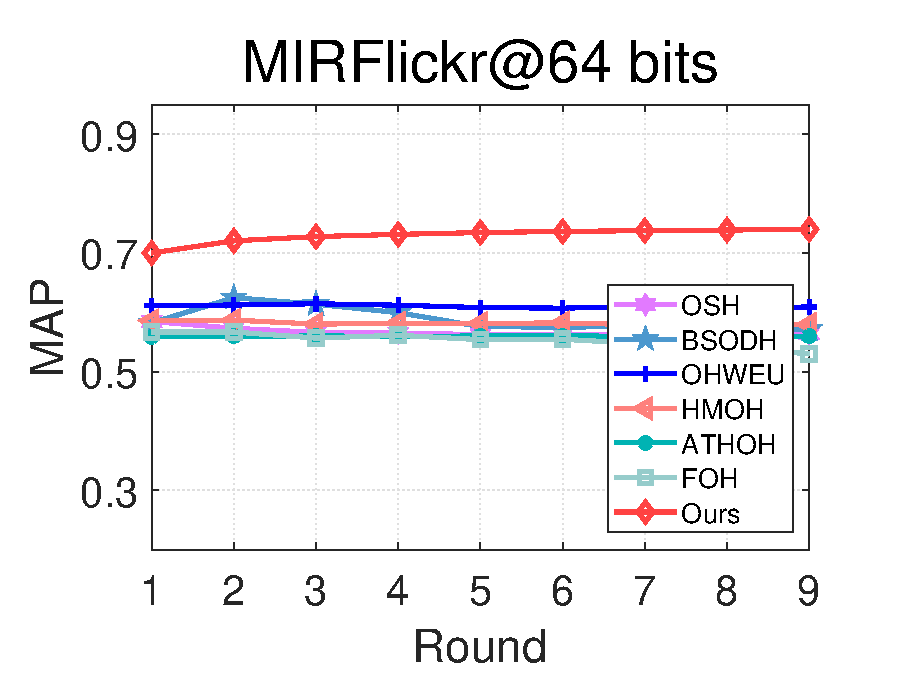
\includegraphics[width=0.3\columnwidth]{figures/map_round/MIRFlickr@64bits}
							\label{fig:MIRFlickr@64bits}} 
						%	\vspace{-2mm}
						\subfloat[]{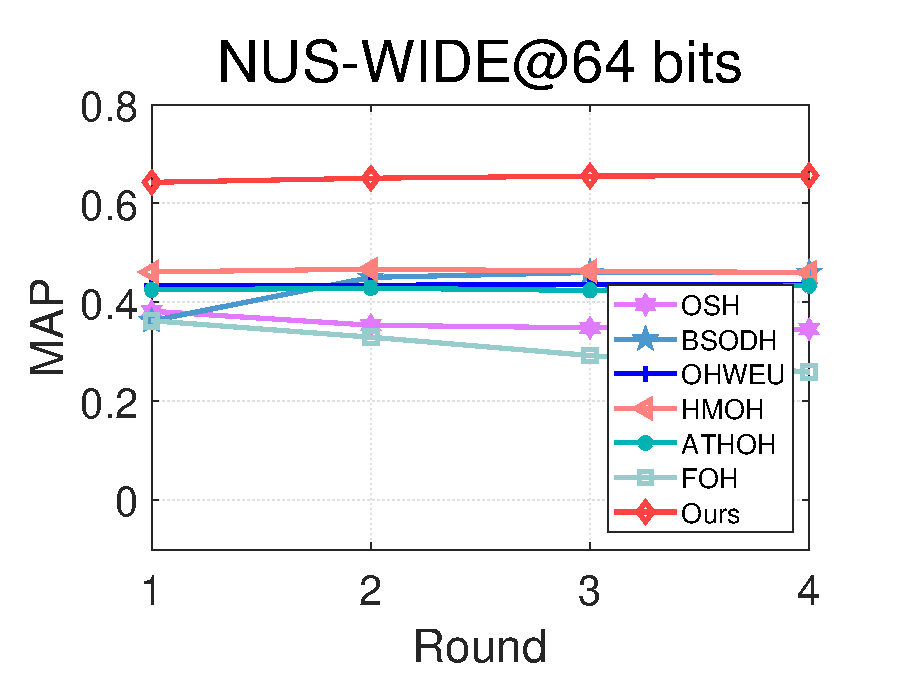
\includegraphics[width=0.3\columnwidth]{figures/map_round/NUS-WIDE@64bits}
							\label{fig:NUS-WIDE@64bits}} 
						%	\vspace{-2mm}
						\caption{The MAP-round curves of on three datasets.}
						\label{fig:map_round}
						\vspace{-6mm}
					\end{figure}
					
					
					\begin{figure}
						\centering
						\captionsetup[subfloat]{labelformat=empty}
						\subfloat[]{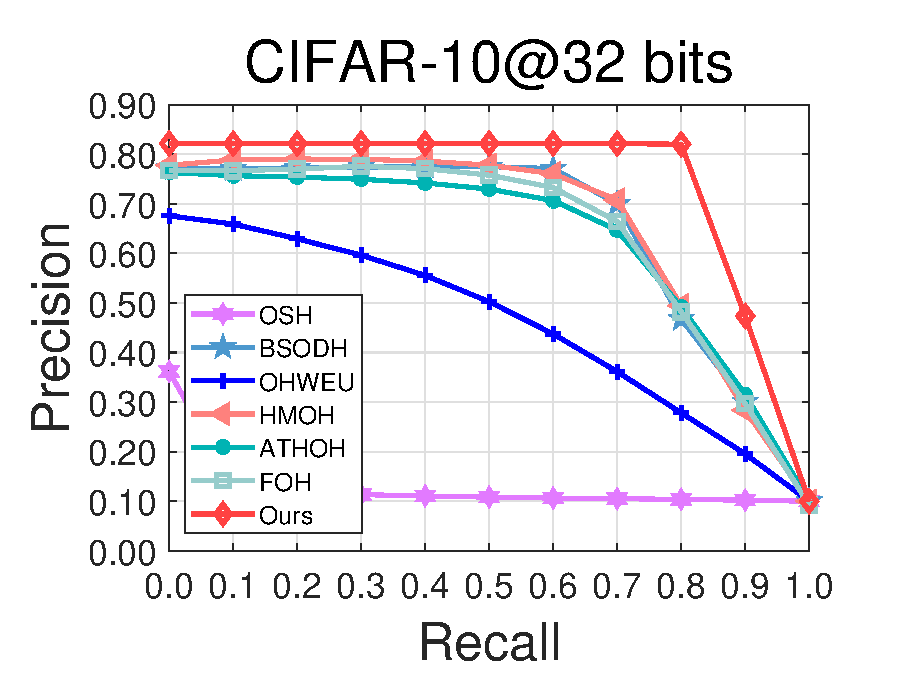
\includegraphics[width=0.3\columnwidth]{figures/pr/CIFAR-10@32bits}
							\label{fig_pr_c_32}}
						\subfloat[]{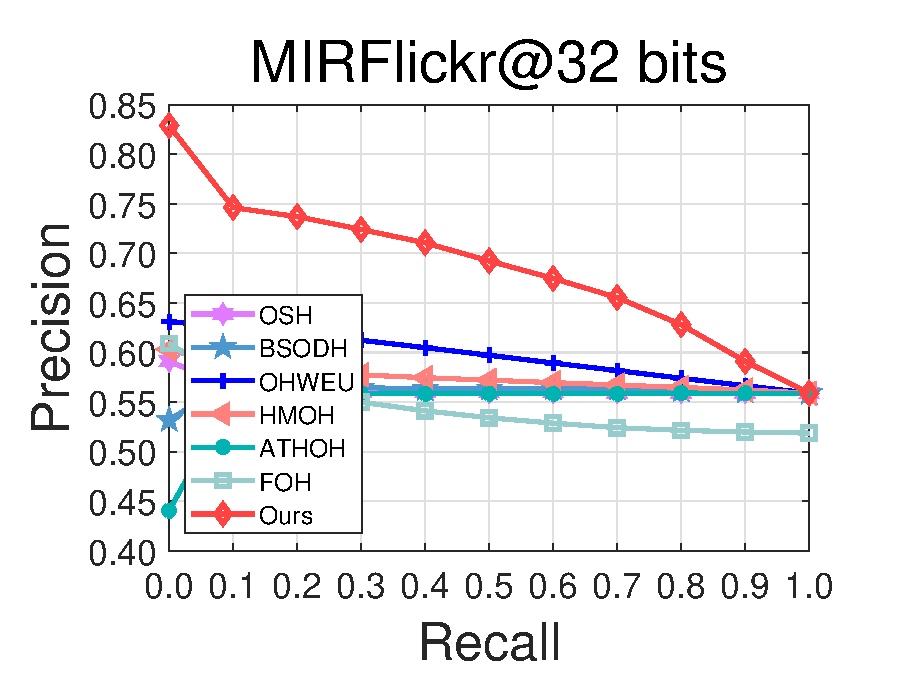
\includegraphics[width=0.3\columnwidth]{figures/pr/MIRFlickr@32bits}
							\label{fig_pr_m_32}}
						\subfloat[]{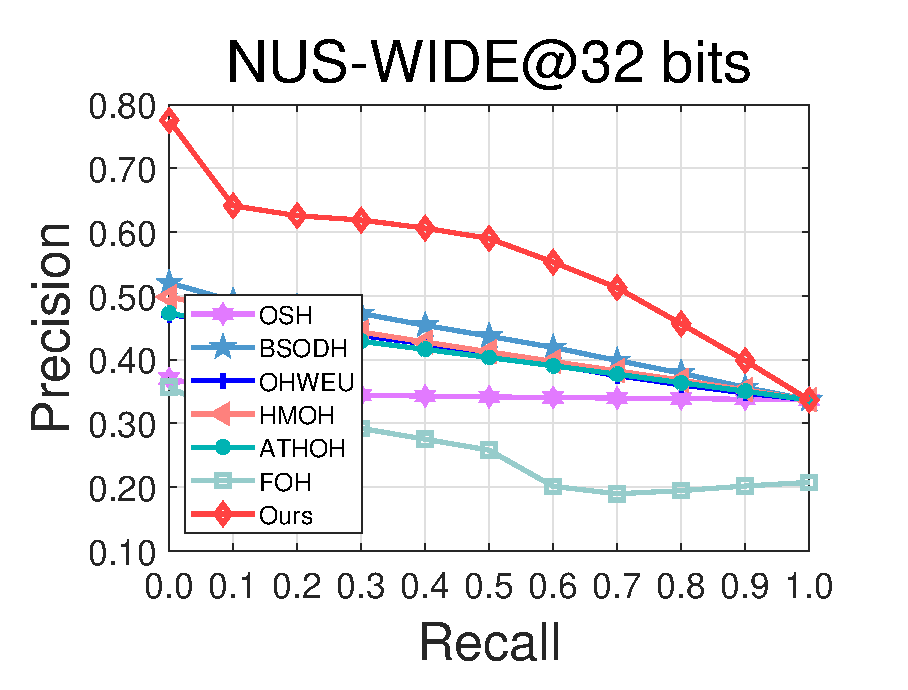
\includegraphics[width=0.3\columnwidth]{figures/pr/NUS-WIDE@32bits}
							\label{fig_pr_n_32}}
						\vspace{-5mm}
						\quad
						\vspace{-5mm}
						\subfloat[]{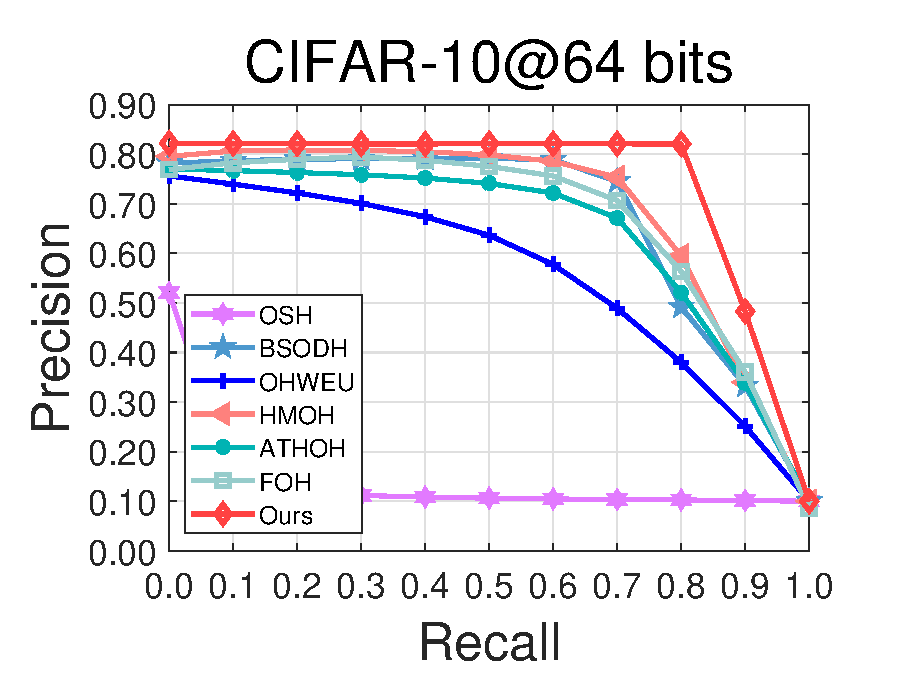
\includegraphics[width=0.3\columnwidth]{figures/pr/CIFAR-10@64bits}
							\label{fig_pr_c_64}}
						%	\vspace{-2mm}
						\subfloat[]{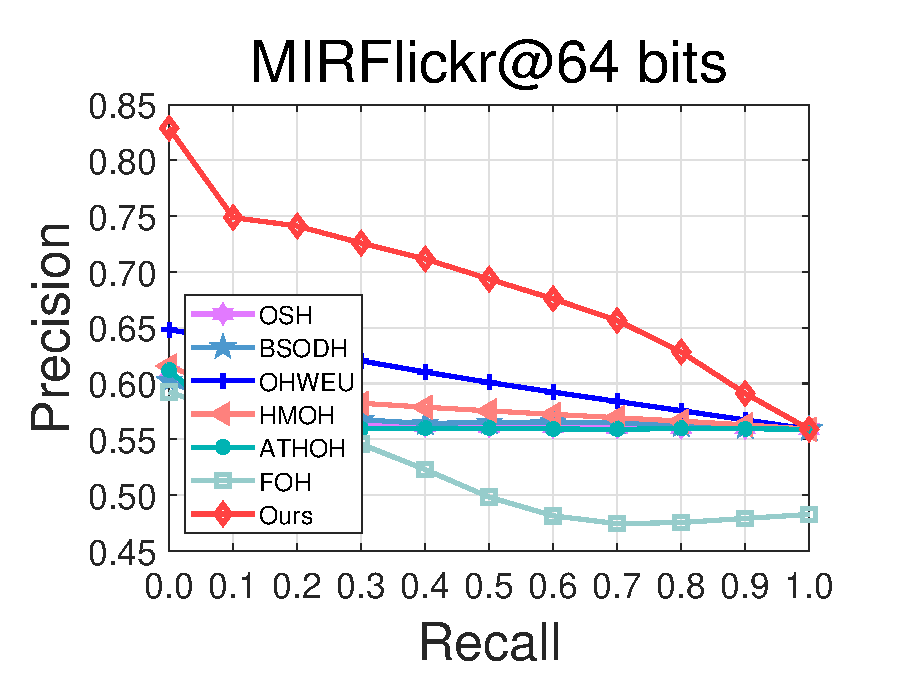
\includegraphics[width=0.3\columnwidth]{figures/pr/MIRFlickr@64bits}
							\label{fig_pr_m_64}} 
						%	\vspace{-2mm}
						\subfloat[]{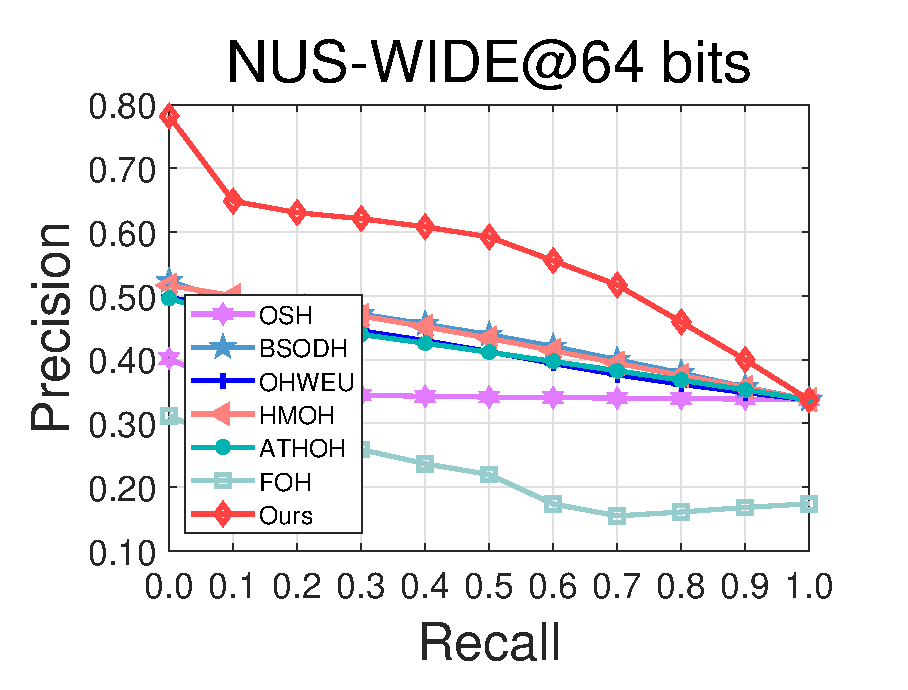
\includegraphics[width=0.3\columnwidth]{figures/pr/NUS-WIDE@64bits}
							\label{fig_pr_n_64}} 
						%	\vspace{-2mm}
						\caption{The precision-recall curves on three datasets.}
						\label{fig:pr_curve}
					\end{figure}
					
					
 					To comprehensively demonstrate the online retrieval performance of our model as streaming data arrives, we plotted the performance of all methods on three datasets with 16-bit and 64-bit hash code lengths  in Fig. \ref{fig:map_round}. Additionally, the precision-recall (P-R) curves of 32 bits and 64 bits hash codes are shown in Fig. \ref{fig:pr_curve}. From these results, we can observe that our proposed method always achieves the best performance in various cases on three datasets, demonstrating the effectiveness of our method. As our proposed method focuses on mitigating catastrophic forgetting, \mymethodname~ could well handle the streaming data and offer satisfying retrieval performance.
 					
 					Please refer more experiments results such as the MAP results of our method and all the comparison methods at last round on three datasets, training time comparison, ablation study, and convergence to our paper, due to the page limit.

					
				\end{block}
				
				\begin{block}{Conclusion}
					
					In this paper, we propose a new online hashing method for streaming data retrieval. \mymethodname~belongs to two-step hashing, containing hash codes learning and hash function learning steps. \mymethodname~has made great efforts for mitigating the catastrophic forgetting. First, we design the learnable hash centers which are guided by both fixed Hadamard-based hash centers and the former hash centers of last round. Then, to embed more knowledge learned from former rounds, exemplars are chosen and stored in exemplar memory. Finally, our hash codes learn from hash centers, exemplars, and the revised hash formulation through the novel overall objective function. To optimize all variables, we present a discrete online optimization with linear complexity, which could learn hash codes accurately and fast. Experimental results on three benchmark datasets demonstrate the effectiveness of both \mymethodname~and functional properties of the multiple components of our method.
				\end{block}
				
				\begin{block}{References}
					
					\nocite{*}
					\footnotesize{\bibliographystyle{plainnat}\bibliography{poster}}
					
				\end{block}
				
			\end{column}
			
			\separatorcolumn
		\end{columns}
	\end{frame}
	
\end{document}